
\begin{frame}
\frametitle{Every odyssey starts with a terrific idea}
\includegraphics[scale=0.30]{img/nextTroy.png}
\end{frame}

\begin{frame}
\frametitle{And utter ignorance of the upcoming complications}
\includegraphics[scale=0.30]{img/bbAndTroy.png}
\end{frame}

\begin{frame}
\frametitle{From dream to reality...}
\includegraphics[scale=0.30]{img/nextCollague.png}
\end{frame}

\begin{frame}
\frametitle{NEXT detector concept}
\includegraphics[scale=0.30]{img/PrincipleNext2.png}
\end{frame}

\begin{frame}
\frametitle{From an empty space}
\includegraphics[scale=0.30]{img/emptyLSC.png}
\end{frame}

\begin{frame}
\frametitle{To a busy place}
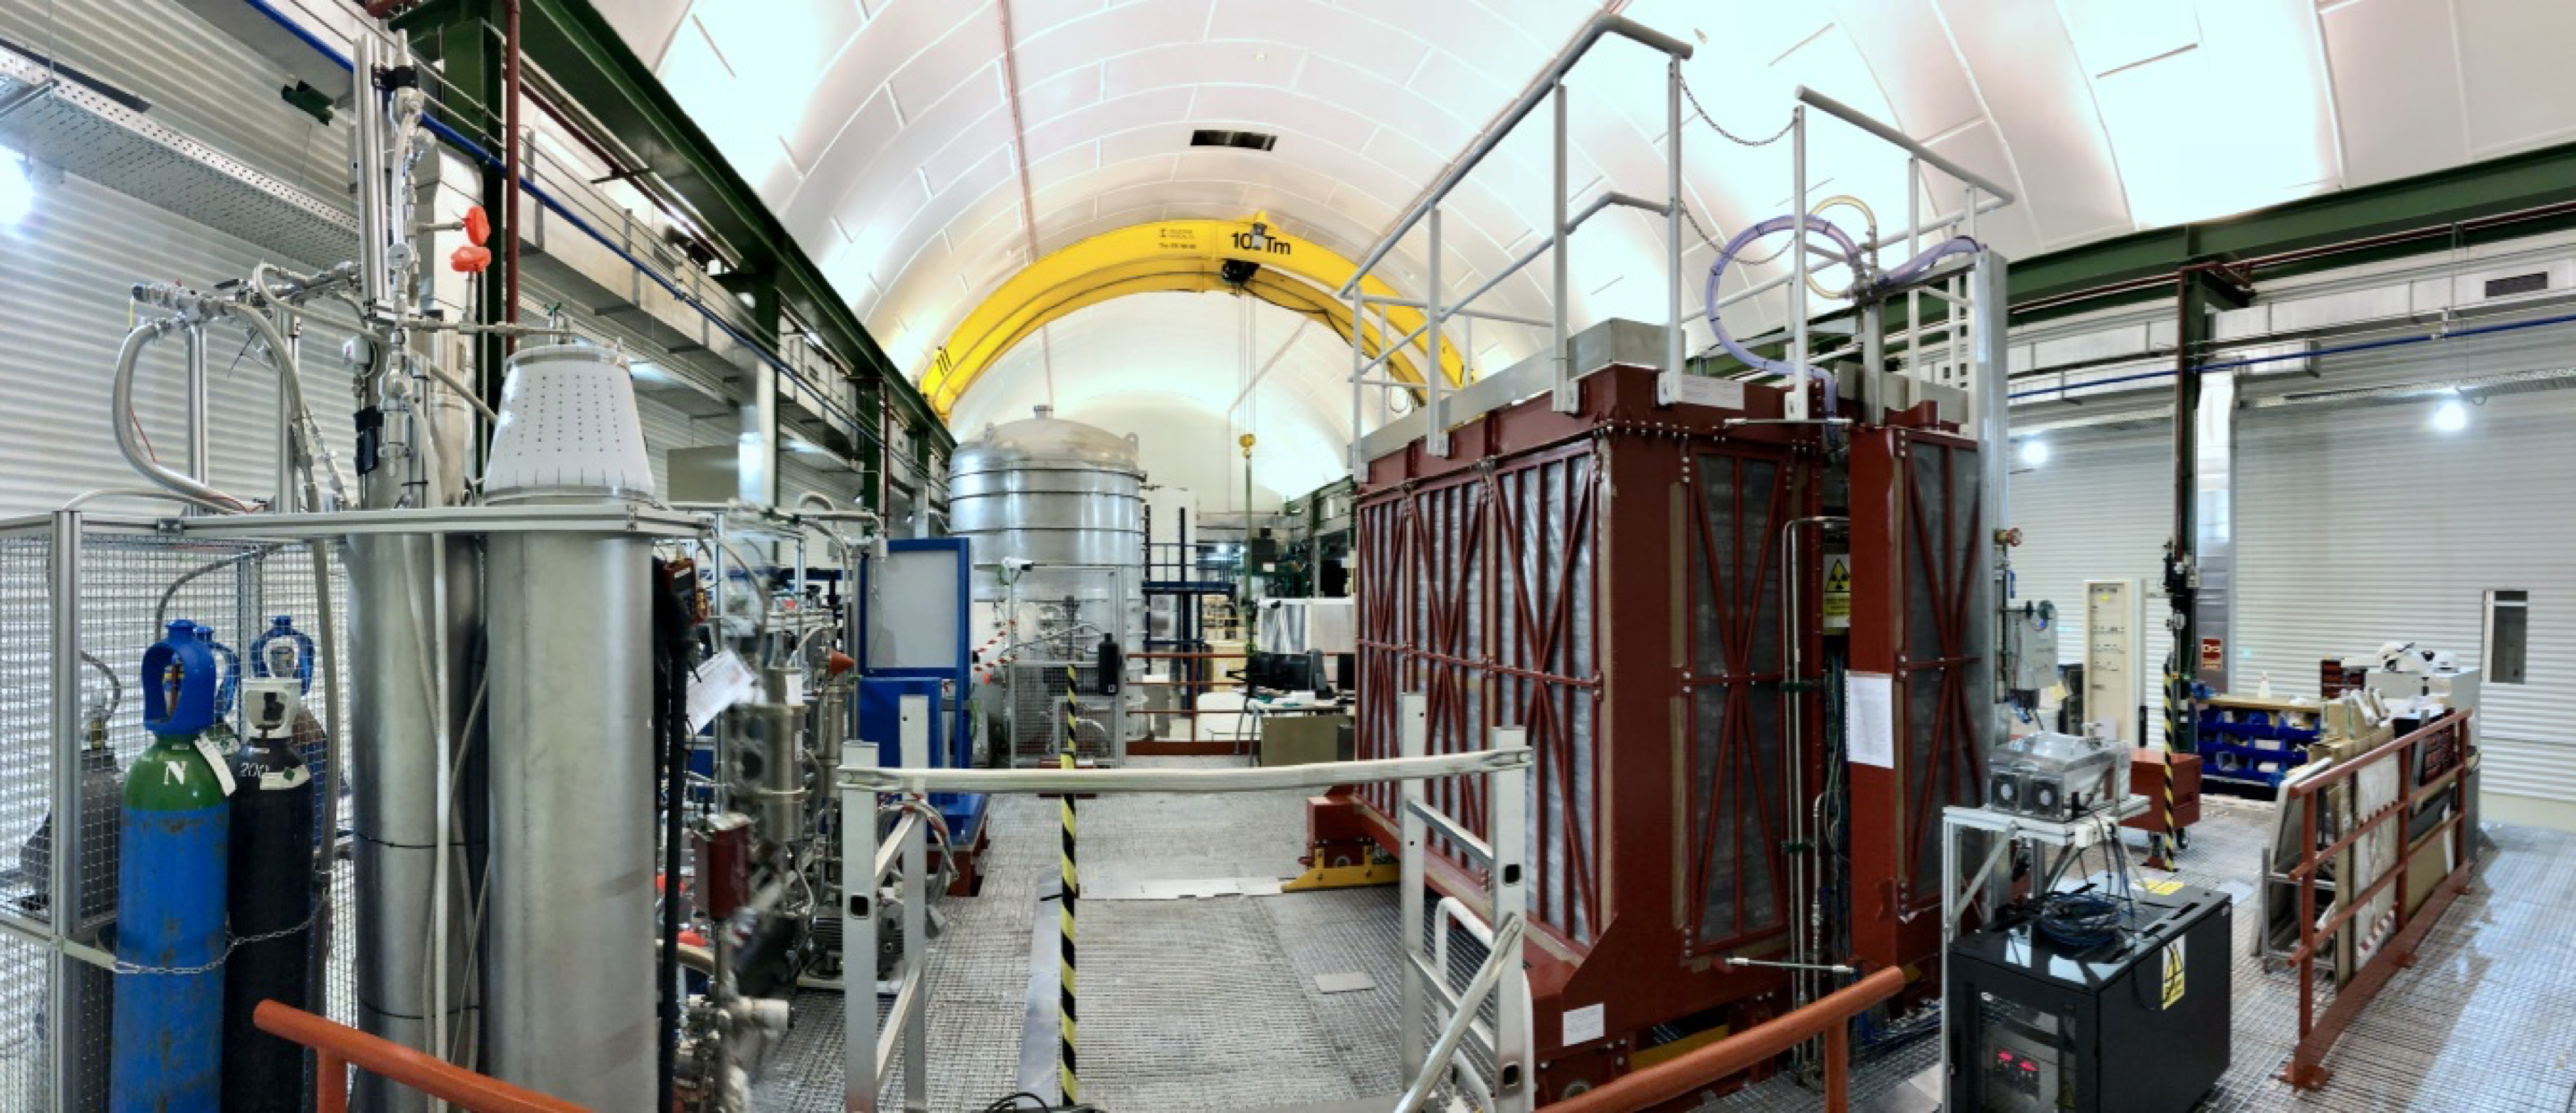
\includegraphics[scale=0.25]{img/lsc2021.png}
\end{frame}

\begin{frame}
\frametitle{Technology works}
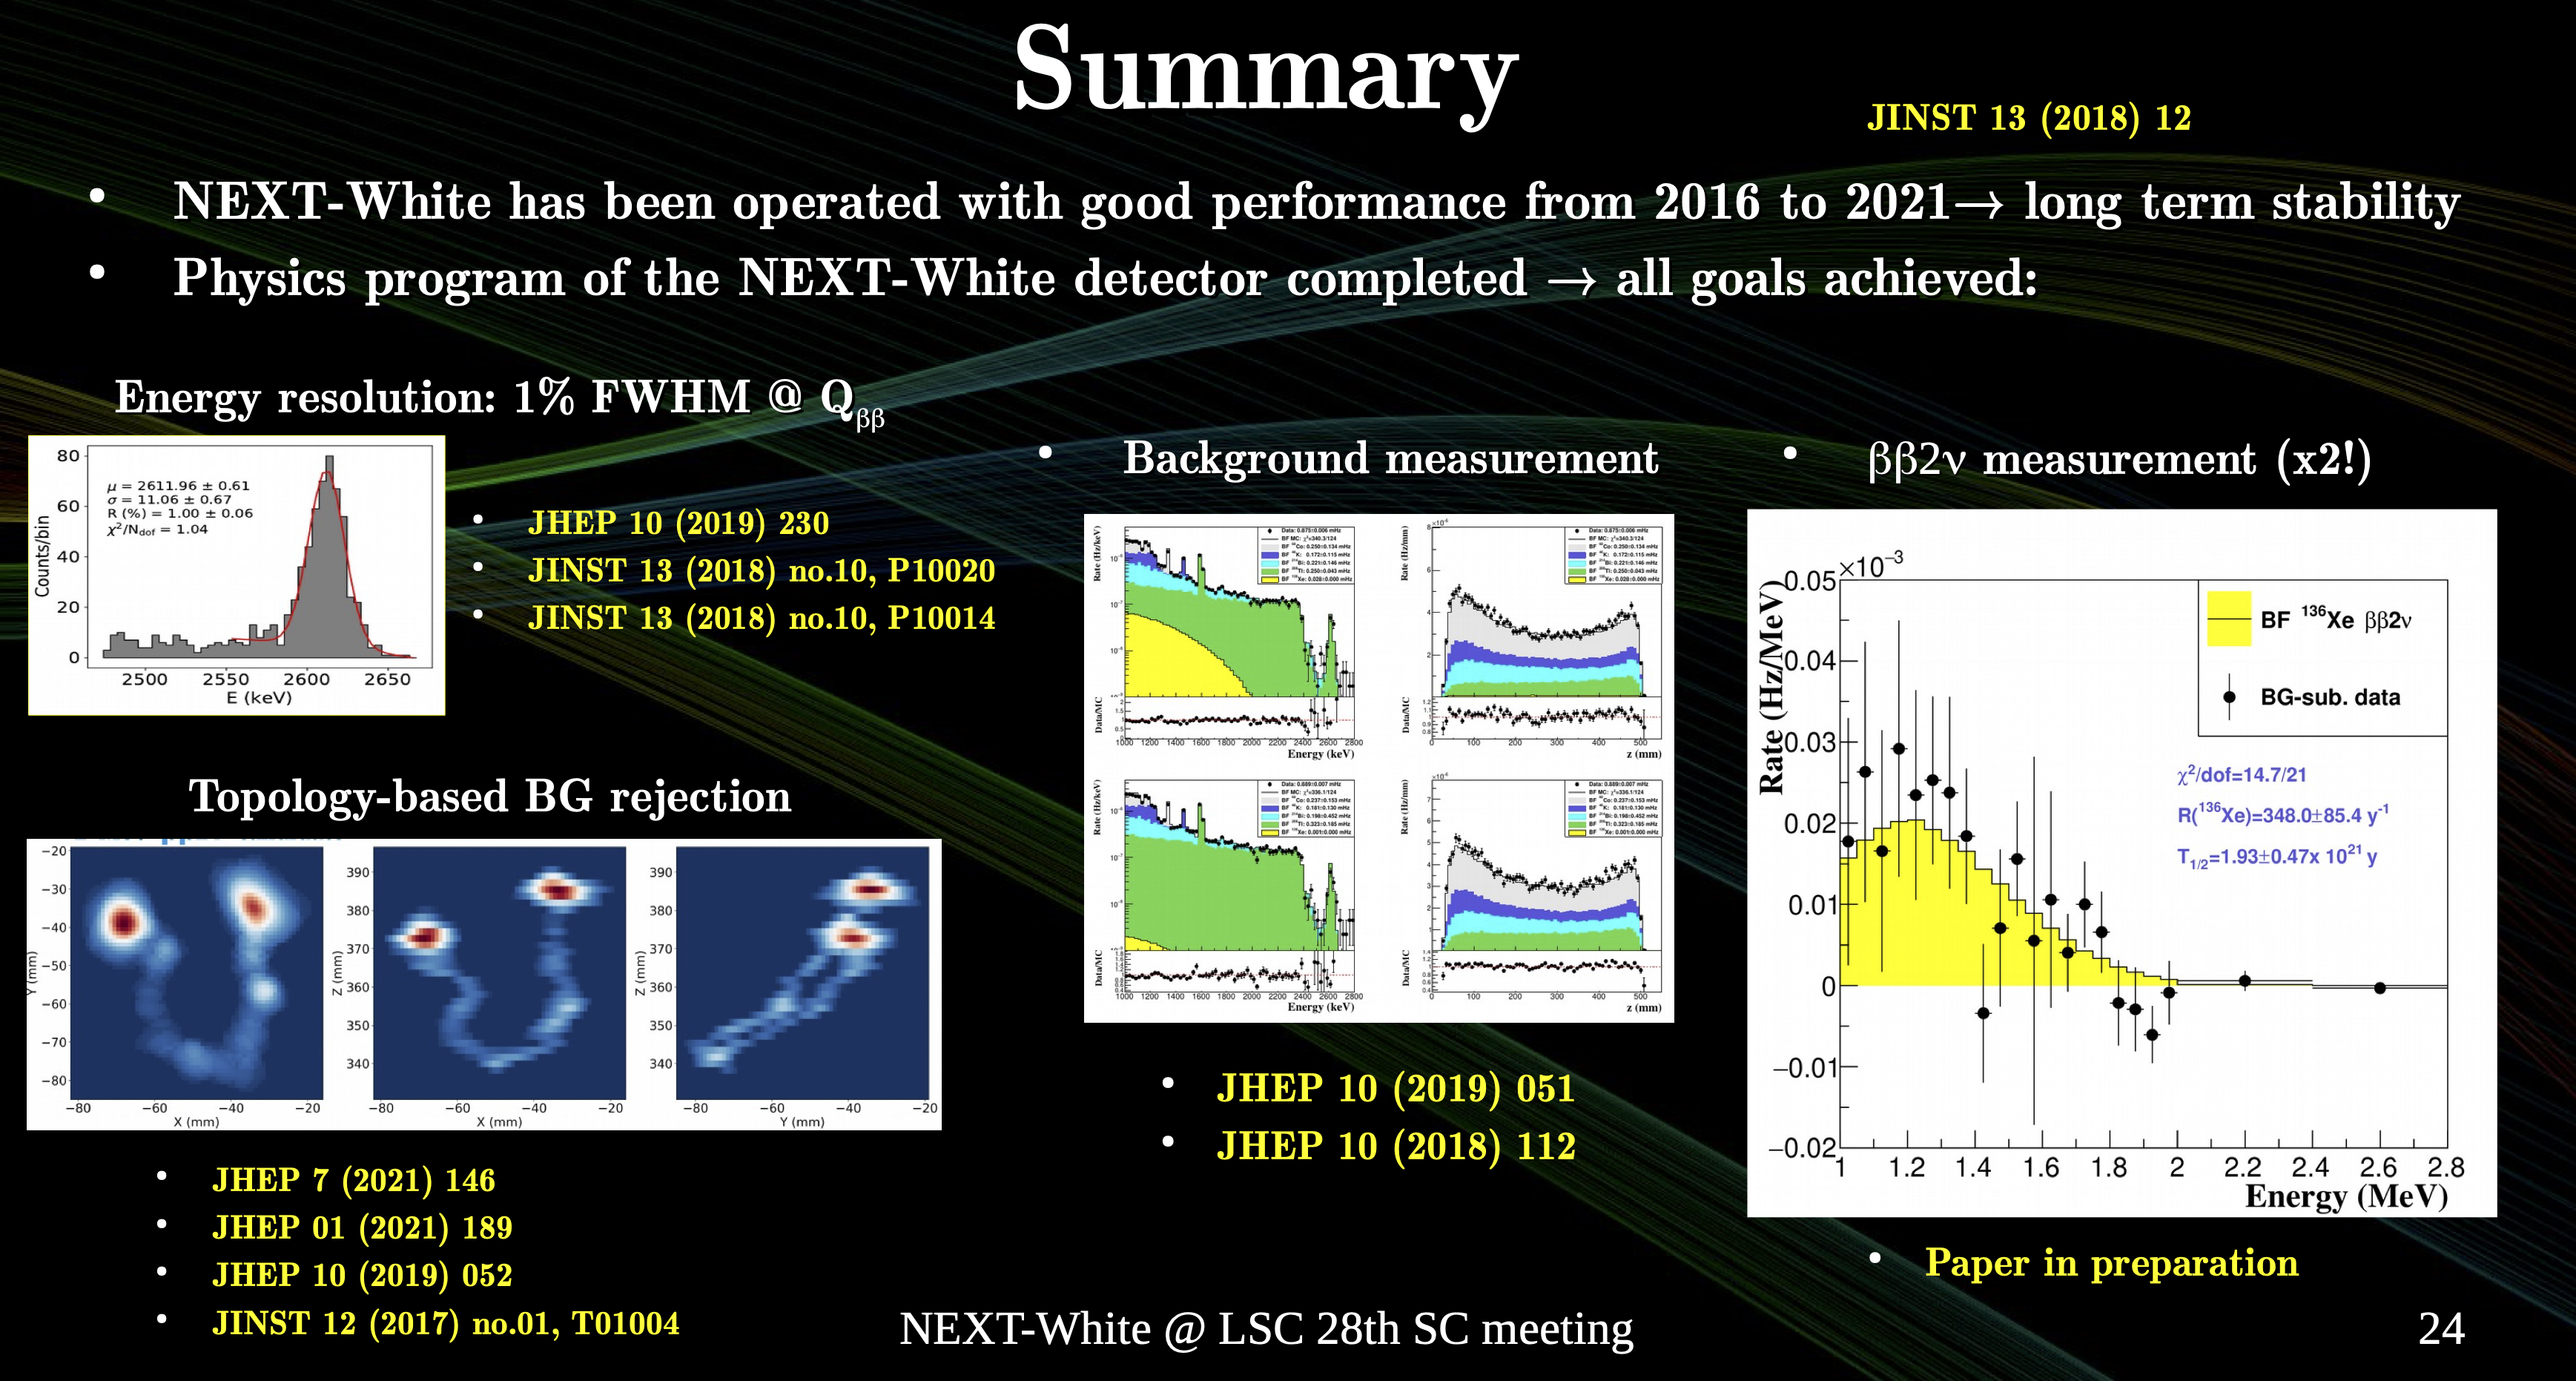
\includegraphics[scale=0.20]{img/whiteResults.png}
\end{frame}

\begin{frame}
\frametitle{But no signal}
\includegraphics[scale=1.00]{img/nosignal.jpg}
\end{frame}

\begin{frame}
\frametitle{From reality to dream}
\includegraphics[scale=0.20]{img/nextProgram.png}
\end{frame}


\begin{frame}
\frametitle{BOLDly go where no one has bone before...}
\begin{columns}
\column{0.45\textwidth}
\includegraphics[scale=0.09]{img/enterprise.jpg}
\column{0.5\textwidth}
$\bullet$~To explore lifetimes of $10^{27}$ y we need an exposure of the order of 1 ton$\cdot$year.

$\bullet$~Thus $10^{28}$ y could be reached achieving exposures of the order of 10 ton$\cdot$year. It could even be that $10^{28}$ y is conceivable. 

$\bullet$~However, this is only possible if we achieve a \alert{fully background free experiment}

$\bullet$~This is the goal of the BOLD project (ERC/Synergy grant, 2020). 

\end{columns}
\end{frame}

\begin{frame}
\frametitle{A new skin for the old ceremony}
\begin{columns}
\column{0.45\textwidth}
\includegraphics[scale=0.2]{img/bariumTagging.png}
\column{0.5\textwidth}
$\bullet$~All current (and planned) $\beta \beta 0 \nu$ experiments detect only the electromagnetic part of the decay (e.g., the electrons). 

$\bullet$~NEXT-BOLD proposed to detect both the electrons and the $Ba^{2+}$ dication. 
 
$\bullet$~Radioactivity produces electrons but not isolated $Ba^{2+}$ dications. 

$\bullet$~But most importantly, we will detect the signal in (delayed) coincidence. \alert{Some trick that allowed the discovery of the neutrino}

\end{columns}
\end{frame}

\begin{frame}
\frametitle{BOLD ingredients}
\begin{columns}
\column{0.45\textwidth}
\includegraphics[scale=0.15]{img/FBI.png}

$\bullet$~Idea (Dave Nygren): Exploit single molecule fluorescent imaging (SFMF) to visualise (“tag”) a  single  $Ba^{2+}$ dication as it arrives at the TPC cathode.

$\bullet$~Fluorescent Bicolor $Ba^{2+}$ sensor (Fernando Coss\'io):Able to trap ("chelate") the dication and change luminous response when this happens. 

\column{0.5\textwidth}
\includegraphics[scale=0.12]{img/nextBold.png}

$\bullet$~Bold Apparatus (JJGC): Capable to detect in delayed coincidence the electron signal (in anode) and the cation signal in cathode.


\end{columns}
\end{frame}

\begin{frame}
\frametitle{A Blue Spark may signal where the grain of sand lies}
\includegraphics[scale=0.18]{img/BaTaResults.png}

\end{frame}


\begin{frame}
\frametitle{Majorana Beach}
\includegraphics[scale=0.30]{img/MajoranaBeach2.png}
\end{frame}
%
%
